\begin{frame}{Foundations for Inference}
    \begin{itemize}
        \item Statistical inference is where we get to take all of the concepts we've learned and use them on our data.
        \item We want to understand and quantify uncertainty related to parameter estimates.
        \item The details will vary, but the foundations will carry you far beyond this class.
    \end{itemize}
\end{frame}

\begin{frame}{Foundations for Inference}
    In this chapter, we will
    \begin{enumerate}
        \item Think about using a sample proportion to estimate a population proportion.
        \item Build confidence intervals, or ranges of plausible values for the population parameter.
        \item Introduce hypothesis testing, which allows us to formally test some of those research questions we talked about in Chapters 1 and 2.
    \end{enumerate}
\end{frame}

\begin{frame}{Point Estimates}
    \begin{itemize}
        \item A recent poll suggests Trump’s approval rating among US adults is 41\%. 
        \item We consider 41\% to be a \textbf{point estimate} for the true approval rating.
        \begin{itemize}
            \item The true rating is what we would see if we could get responses from every single adult in the US. 
        \end{itemize}
        \item The response from the entire population is the \textbf{parameter} of interest.
    \end{itemize}
\end{frame}

\begin{frame}{Point Estimates}
    \begin{itemize}
        \item When the parameter is a proportion, it is often denoted by $p$.
        \item The sample proportion is denoted $\hat{p}$ (p-hat). 
        \item Unless we collect responses from every individual in the population, $p$ is unknown.
        \item We use $\hat{p}$ as our estimate of $p$. 
    \end{itemize}
\end{frame}

\begin{frame}{Sampling Distribution}
    \begin{tabular}{c|c|c}
        Sample \# & Observations & Mean  \\
        \hline
        1 & $x_{1,1}$ $x_{1,2}$ \dots $x_{1,n}$ & $\bar{x}_1$ \\
        2 & $x_{2,1}$ $x_{2,2}$ \dots $x_{2,n}$ & $\bar{x}_2$ \\
        3 & $x_{3,1}$ $x_{3,2}$ \dots $x_{3,n}$ & $\bar{x}_3$ \\
    \end{tabular}
    \\ Etc.
    
    \vspace{12pt}$\bar{x}$ will change each time we get a new sample. Therefore, when $x$ is a random variable, $\bar{x}$ is also a random variable. (Recall that we also estimate $p$ by $\hat{p} =\bar{x}$.)
\end{frame}

\begin{frame}{Error}
    \begin{itemize}
        \item The difference between the sample proportion and the parameter is called the \textbf{error} in the estimate. 
        \item Error consists of two aspects: 
        \begin{enumerate}
            \item sampling error 
            \item bias.
        \end{enumerate}
    \end{itemize}
\end{frame}

\begin{frame}{Sampling error}
    \begin{itemize}
        \item \textbf{Sampling error} is how much an estimate tends to vary between samples.
        \item This is also referred to as \textit{sampling uncertainty}.
        \item E.g., in one sample, the estimate might be 1\% above the true population value. 
        \item In another sample, the estimate might be 2\% below the truth. 
        \item Our goal is often to quantify this error. 
    \end{itemize}
\end{frame}

\begin{frame}{Bias}
    \begin{itemize}
        \item \textbf{Bias} is a \textit{systematic} tendency to over- or under-estimate the population true value.
        \item E.g., Suppose we were taking a student poll asking about support for a UCR football team.
        \item Depending on how we phrased the question, we might end up with very different estimates for the proportion of support.
        \item We try to minimize bias through thoughtful data collection procedures.
    \end{itemize}
\end{frame}

\begin{frame}{Variability of a Point Estimate}
    \begin{itemize}
        \item Suppose the true proportion of American adults who support the expansion of solar energy is $p = 0.88$
        \begin{itemize}
            \item This is our parameter of interest.
        \end{itemize}
        \item If we took a poll of 1000 American adults, we wouldn't get a perfect estimate.
        \item Assume the poll is well-written (unbiased) and we have a random sample. 
    \end{itemize}
\end{frame}

\begin{frame}{Variability of a Point Estimate}
    \begin{itemize}
        \item How close might the sample proportion ($\hat{p}$) be to the true value?
        \item We can think about this using simulations. 
        \item This is possible because we know the true proportion to be $p=0.88$.
    \end{itemize}
\end{frame}

\begin{frame}{Variability of a Point Estimate}
    Here’s how we might go about constructing such a simulation:
    \begin{enumerate}
        \item There were about 250 million American adults in 2018. On 250 million pieces of paper, write “support” on 88\% of them and “not” on the other 12\%.
        \item Mix up the pieces of paper and randomly select 1000 pieces to represent our sample of 1000 American adults.
        \item Compute the fraction of the sample that say “support”.
    \end{enumerate}
\end{frame}

\begin{frame}{Variability of a Point Estimate}
    \begin{itemize}
        \item Obviously we don't want to do this with paper, so we will use a computer.
        \item Using \texttt{R}, we got a point estimate of $\hat{p}_1=.894$.
        \item This means that we had an error of $0.894 − 0.88 = +0.014$
    \end{itemize}
    Note: the \texttt{R} code for this simulation may be found on page 171 of the textbook. 
\end{frame}

\begin{frame}{Variability of a Point Estimate}
    \begin{itemize}
        \item This code will give a different estimate each time it's run (so the error will change each time).
        \item Therefore, we need to run multiple simulations.
        \item In more simulations, we get
        \begin{enumerate}
            \item $\hat{p}_2 = 0.885$, which has an error of $+0.005$
            \item $\hat{p}_3 = 0.878$ with an error of $-0.002$
            \item $\hat{p}_4 = 0.859$ with an error of $-0.021$
        \end{enumerate}
    \end{itemize}
\end{frame}

\begin{frame}{Variability of a Point Estimate}
    \begin{center}
        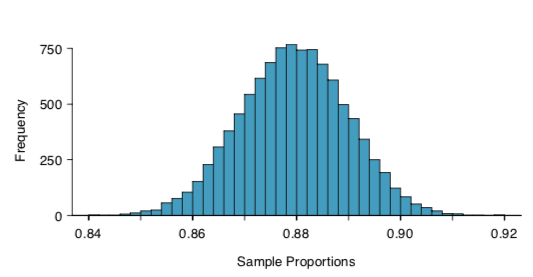
\includegraphics[scale=0.5]{images/samplingdist.png}
    \end{center}
    \vspace{-10pt}The histogram shows the estimates across 10,000 simulations. This distribution of sample proportions is called a \textbf{sampling distribution}.
\end{frame}

\begin{frame}{Sampling Distribution}
    We can characterize this \textit{sampling distribution} as follows:
    
    \vspace{12pt}\textbf{Center}:
    \begin{itemize}
        \item  The center is $\bar{x}_{\hat{p}}=0.880$, the same as our parameter.
        \item This means that our estimate is unbiased.
        \item The simulations mimicked a simple random sample, an approach that helps avoid bias.
    \end{itemize}
\end{frame}

\begin{frame}{Sampling Distribution}
    We can characterize this sampling distribution as follows:
    
    \vspace{12pt}\textbf{Spread}. 
    \begin{itemize}
        \item The standard deviation of the sampling distribution is $s_{\hat{p}} = 0.010$.
        \item When we’re talking about a sampling distribution or the variability of a point estimate, we use the term \textbf{standard error} instead of standard deviation. 
        \item Standard error for the sample proportion is denoted $SE_{\hat{p}}$.
    \end{itemize}
\end{frame}

\begin{frame}{Sampling Distribution}
    We can characterize this sampling distribution as follows:
    
    \vspace{12pt}\textbf{Shape}. 
    \begin{itemize}
        \item The distribution is symmetric and bell-shaped - it resembles a normal distribution.
    \end{itemize}
    
    \vspace{12pt}These are all good! When the population proportion is $p = 0.88$ and the sample size is $n = 1000$, the sample proportion $\hat{p}$ is a good estimate \textit{on average}.
\end{frame}

\begin{frame}{Sampling Distribution}
    Note that the sampling distribution is never observed! 
    
    \vspace{12pt}However,
    \begin{itemize}
        \item It is useful to think of a point estimate as coming from a distribution.
        \item The sampling distribution will help us make sense of the point estimates that we do observe.
    \end{itemize}
\end{frame}

\begin{frame}{Example}
    What do you think would happen if we had a sample size of 50 instead of 1000?
    
    \begin{itemize}
        \item Intuitively, more data is better.
        \item This is true!
        \item If we have less data, we expect our sampling distribution to have higher variability.
        \item In fact, the standard error will increase if we decrease sample size.
    \end{itemize}
\end{frame}

\begin{frame}{Central Limit Theorem}
    \begin{itemize}
        \item The sampling distribution histogram we saw looked a lot like a normal distribution.
        \item This is no coincidence!
        \item This is the result of a principle called the \textbf{Central Limit Theorem}.
    \end{itemize}
\end{frame}

\begin{frame}{Central Limit Theorem}
    When observations are independent and the sample size is sufficiently large, the sample proportion $\hat{p}$ will tend to follow a normal distribution with mean
    \[
        \mu_{\hat{p}} = p
    \]
    and standard error
    \[
        SE_{\hat{p}} = \sqrt{\frac{p(1-p)}{n}}
    \]
\end{frame}

\begin{frame}{The Success-Failure Condition}
    In order for the Central Limit Theorem to hold, the sample size is typically considered sufficiently large when 
    \[
        np \ge 10
    \]
    and 
    \[
        n(1 − p) \ge 10
    \]
    \vspace{12pt}This is called the \textbf{success-failure condition}.
\end{frame}

\begin{frame}{Standard Error}
    Using the standard error, we can see that the variability of a sampling distribution \textit{decreases} as sample size \textit{increases}.
    \[
        SE_{\hat{p}} = \sqrt{\frac{p(1-p)}{n}}
    \]
\end{frame}

\begin{frame}{Example}
    Confirm that the Central Limit Theorem applies for our example with $p=0.88$ and $n=1000$. Confirm that the Central Limit Theorem applies.
\end{frame}

\begin{frame}{Example}
    \textbf{Independence}. There are $n = 1000$ observations for each sample proportion $\hat{p}$, and each of those observations are independent draws. 
    
    \begin{itemize}
        \item The most common way for observations to be considered independent is if they are from a simple random sample.
        \item If a sample is from a seemingly random process, checking independence is more difficult. Use your best judgement.
    \end{itemize}
\end{frame}

\begin{frame}{Example}
    \textbf{Success-failure condition}. 
    
    \[
        np = 1000 \times 0.88 = 880 \ge 10
    \]
    and
    \[
        n(1 − p) = 1000 \times (1 − 0.88) = 120 \ge 10
    \]
    The independence and success-failure conditions are both satisfied, so the Central Limit Theorem applies and it’s reasonable to model $\hat{p}$ using a normal distribution.
\end{frame}

\begin{frame}{Example}
    Compute the theoretical mean and standard error of $\hat{p}$ when $p = 0.88$ and $n = 1000$, according to the Central Limit Theorem.
    \[
        \mu_{\hat{p}} = p = 0.88
    \]
    and
    \[
        SE_{\hat{p}} = \sqrt{\frac{p(1-p)}{n}} = \sqrt{\frac{0.88\times(1-0.88)}{1000}} = 0.010
    \]
    \vspace{12pt}So $\hat{p}$ is distributed approximately $N(0.88, 0.010)$.
\end{frame}

\begin{frame}{Example}
    Estimate how frequently the sample proportion $\hat{p}$ should be within 0.02 of the population value, $p = 0.88$.
\end{frame}

\begin{frame}{Example}
    Within 0.02 of 0.88 is between $0.86$ and $0.90$. As before, we will find the Z-scores.
    \[
        z_{0.86} = \frac{0.86-0.88}{0.010} = -2
    \]
    and 
    \[
        z_{0.90} = \frac{0.90-0.88}{0.010} = 2
    \]
\end{frame}

\begin{frame}{Example}
    Using software,
    \begin{align*}
        P(-2 < Z < 2) &= 1 - P(Z > 2) - P(Z < -2) \\
        &= P(Z < 2) - P(Z < -2) \\
        &= 0.977 - 0.023 \\
        &= 0.954
    \end{align*}
    So 95.4\% of the proportions should fall within 0.02 of the true population value. 
\end{frame}

\begin{frame}{Central Limit Theorem in the Real World}
    \begin{itemize}
        \item In a real-world setting, we almost never know the true population proportion. 
        \item However, we use the population proportion to determine whether the Central Limit Theorem is appropriate. 
        \item How do we verify use of the Central Limit Theorem?
    \end{itemize}
\end{frame}

\begin{frame}{Central Limit Theorem in the Real World}
    Independence. The poll is a simple random sample of American adults, which means that the observations are independent.

    \vspace{12pt}Success-failure condition. Without the population proportion, we use $\hat{p}$ as our next best way to check the success-failure condition.
    \[
        n\hat{p} \ge 10
    \]
    and
    \[
        n(1-\hat{p}) \ge 10
    \]
\end{frame}

\begin{frame}{Central Limit Theorem in the Real World}
    We call this a \textbf{substitution approximation} or the \textit{plug-in principle}. 
    
    \vspace{12pt}This can also be used to estimate the standard error:
    \[
        SE{\hat{p}} \approx \sqrt{\frac{\hat{p}(1-\hat{p})}{n}}
    \]
    
    \vspace{12pt}This estimate of the standard error tends to be a good approximation of the true standard error.
\end{frame}

\begin{frame}{More About the Central Limit Theorem}
    What is our conditions don't hold and either
    \[
        np < 10
    \]
    or 
    \[
        n(1-p) < 10?
    \]
\end{frame}

\begin{frame}{More About the Central Limit Theorem}
    Let's do another simulation. Suppose $p=0.25$. Here’s a sample of size $n=10$:
    \[
        \text{no, no, yes, yes, no, no, no, no, no, no}
    \]
    Here, $\hat{p}=0.2$ for yeses. 
\end{frame}

\begin{frame}{More About the CLT}
    Notice that
    \[
        np = 10\times0.25=2.5 < 10
    \]
    The mean and standard deviation for this binomial distribution are $2.5$ and $0.137$, respectively.
    
    \vspace{12pt}If we simulate many samples with $n=10$ and $p=0.25$, what happens to the sampling distribution?
\end{frame}

\begin{frame}{More About the CLT}
    \begin{center}
        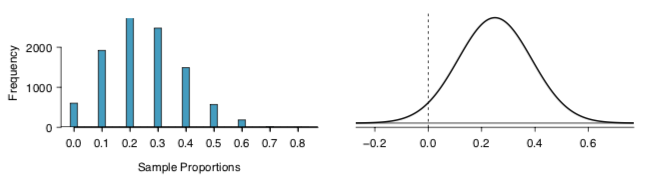
\includegraphics[scale=0.5]{images/sampdist2.png}
    \end{center}
    \begin{itemize}
        \item The histogram shows simulations of $\hat{p}$ for $n=10$ and $p=0.25$
        \item The normal distribution has the same mean (0.25) and standard deviation (0.137).
    \end{itemize}
\end{frame}

\begin{frame}{More About the CLT}
    \begin{center}
        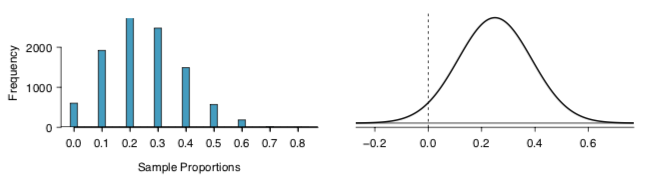
\includegraphics[scale=0.5]{images/sampdist2.png}
    \end{center}
    \begin{itemize}
        \item The normal distribution is unimodal, smooth, and symmetric.
        \item The sampling distribution is unimodal, but it is neither smooth nor symmetric.
    \end{itemize}
\end{frame}

\begin{frame}{More About the CLT}
    In general, when $np$ or $n(1-p)$ are less than 10,
    \begin{itemize}
        \item The distribution is not continuous.
        \item The skew is more noteworthy.
    \end{itemize}
    When $np$ and $n(1-p)$ are greater than 10,
    \begin{itemize}
        \item The larger both $np$ and $n(1−p)$, the more normal the distribution.
    \end{itemize}
\end{frame}

\begin{frame}{More About the CLT}
    \begin{itemize}
        \item The sampling distribution is always centered at the true population proportion $p$ (i.e., $\mu=p$).
        \item This means that the sample proportion $\hat{p}$ is an \textit{unbiased} estimate of $p$.
        \begin{itemize}
            \item This is true as long as the data are independent.
        \end{itemize}
    \end{itemize} 
\end{frame}

\begin{frame}{More About the CLT}
    \begin{itemize}
        \item The variability decreases as the sample size $n$ increases.
        \item Remember our formula for standard error!
        \item Estimates based on a larger sample are intuitively more likely to be accurate.
    \end{itemize}
\end{frame}

\begin{frame}{More About the CLT}
    \begin{itemize}
        \item For a particular sample size, the standard error is largest when $p=0.5$
        \item This is also reflected in the standard error formula.
    \end{itemize}
    \[
        SE_{\hat{p}} = \sqrt{\frac{p(1-p)}{n}}
    \]
    $p(1-p)$ is maximized at $p=0.5$.
\end{frame}

\begin{frame}{More About the CLT}
    \begin{itemize}
        \item The distribution of $\hat{p}$ will always be discrete.
        \item However, the normal distribution is still a good \textit{approximation} when the success-failure condition holds.
    \end{itemize}
    There are about 25 examples of sampling distributions with different values of $n$ and $p$ on pages 176 and 177 of the textbook.
\end{frame}

\begin{frame}{Extending the Framework}
    \begin{itemize}
        \item Using a sample statistic to estimate a parameter is quite common.
        \item We can apply this to many other statistics (other than proportions).
        \item The mean is also a very common statistic and parameter.
        \item In this case, we use $\bar{x}$ to estimate $\mu$.
    \end{itemize}
    We will talk more about estimation strategies for the mean in another chapter. 
\end{frame}